\chapter{Conclusions}
\label{cha:conclusions}

This project combines the strongest of several \textbf{open-source} components: KDL, Ceres Solves, ROS, OpenCV and PR2 (open-source platform, see Figure \ref{fig:PR2_free_robot}). It cannot be less to contribute in the same way to the community, making the code freely available as a ROS package (even though it is still in development stage).

\begin{figure}[!htbp]
 \centering
 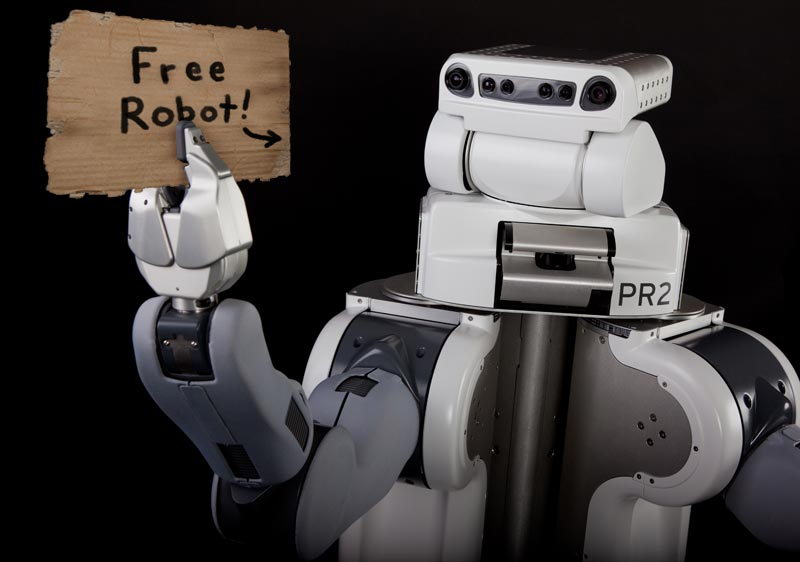
\includegraphics[width=0.6\textwidth]{images/PR2_free_robot.jpg}
 \caption{PR2 pleased to be free.}
 \label{fig:PR2_free_robot}
\end{figure}

The above mentioned software components are well designed, with excellent interfaces and documentation. Even though this fact, \textbf{combining} them in an unique product is a \textbf{time consuming} task, which requires different type of abilities; for example, solve compilation problems with CMake or Catkin (new compilation system in ROS), to mention one.

Regarding the thesis itself, two different methods have been proposed for the \textbf{structure initialization} (3D points). Initialization used for the bundle adjustment optimizer (Ceres Solver). These methods are: solvePnP --3D points in the camera reference-- and the n-view triangulation method.

The improvement in calibration has been shown \textbf{visually} --for a human-friendly comparison-- and \textbf{quantitatively} --for a more rigorous analysis--. A bias has been observed in the solvePnP solution, which will lead in further investigations using the second method (n-view triangulation), with the intention of improving even more the results.

\textbf{Robot calibration} is an important problem to be solved in any robot, in order to allow an effective interaction with the environment. This thesis has been focused in \textbf{multiple camera calibration}. The work has been done experimenting with real data, real robot, real problems.


To conclude this thesis, it has been a total \textbf{proud} to work with two excellent person like David Fofi and Vincent Rabaud, and in two excellent places like Le2i and Willow Garage.
